\documentclass[11pt,a4paper]{article}
\usepackage[latin1]{inputenc}
\usepackage{amsmath}
\usepackage{amsfonts}
\usepackage{amssymb}
\usepackage{graphicx}
\usepackage[left=1.80cm, right=1.80cm, top=2.00cm, bottom=2.00cm]{geometry}
\usepackage{times}
\usepackage[font=small, labelfont=bf]{caption}
\usepackage{subcaption}
\author{Janmejoy Sarkar}
\title{LED based flat-field for pixel to pixel response correction of SUIT CCD.}
\begin{document}
\begin{center}
	\Large {\textbf{LED based flat-field for pixel to pixel response correction of SUIT CCD.}}
	
	\small Note prepared by Janmejoy Sarkar on behalf of SUIT team | \today
\end{center}
\hrule
\section{Introduction}
	The photometric response of an imaging system can vary spatially across its field of view. This can occur due to several reasons such as vignette, non-uniform response across the image sensor, dust or other contaminants within the beam path, etc. This non uniformity can be large scale- ranging over tens or hundreds of pixels, or could small scale arising due to the non uniform quantum efficiciency of each pixel in the image sensor. To perform reliable photometry, it is necessary to understand the profile of this non uniformity and to remove it,  which is achieved by dividing a flat field image from the data. Therefore, flat field correction is of utmost importance for SUIT.
	
	The large scale photometric variation of SUIT shall be modeled by placing a standard star like Sirius at various field angles. The SUIT field of view has been tested interferometrically and no vignette is seen within a  region of $\pm 23~mm (\pm 22 ~arcmin)$ on both X and Y axes at the CCD plane. Therefore, no portion of the solar disc shall be vignetted, even if SUIT is pointed at an offset of 2 arcmin with respect to VELC. The small scale, pixel-to-pixel response variation will however be modeled using LEDs placed on board the payload. This document presents the methodology for pixel-to-pixel flat field correction using on board LEDs, optimizes the correction procedure, presents the generated results and demonstrates the efficacy of the process with simulated images.
	
	
\section{Methodology} 
	\begin{enumerate}
		\item \textbf{LED images:} Multiple LED images are recorded with SUIT in one particular filter combination. Several such images are added, after bias subtraction, to increase the signal to noise ratio and prepare a parent image.	The parent image has a large scale feature dependent on the mode of illumination along with pixel to pixel variation in response, which we are interested to find. 
	
	For a pixel at location $(i,j)$, the photoelectrons generated in each pixel ($P_{ij}$) would be given by-
	
	\begin{equation}
		P_{ij} = S_{ij}\cdot k_{ij}  \label{Pij}
	\end{equation}
	where $ S_{ij} $ represents the photoelectrons due to LED illumination and $k_{ij}$ represents $(i,j)^{th}$ pixel response.
	
	The variation of $ S_{ij} $ over a small region is negligible as the LED illumination produces a large scale pattern. Therefore, $S_{i,j}$ is invariant at pixel ($i+\Delta i, j+\Delta j$)  for small $\Delta i, \Delta j$.
	\begin{align}
		S_{ij}= S_{i+\Delta i, j + \Delta j} = S
	\end{align}  
	
	For small $\Delta i, \Delta j$, we get from Eqn. \ref{Pij}-
	\begin{align}
		P_{i+\Delta i, j + \Delta j}&= S \cdot k_{i+\Delta i, j + \Delta j}\\
	\end{align}
	Therefore, we can also say-
	
	\begin{equation}
		P_{ij} = S\cdot k_{ij}
	\end{equation}
	
	\item \textbf{Flat Field Generation:} The Parent image is now blurred by Boxcar convolution method.  The kernel size is so chosen as to preserve the large scale pattern while removing the small scale pattern as much as possible. 
		
	Upon performing a boxcar convolution with a kernel of size ($\Delta i, \Delta j$) on the parent image, each pixel assumes the average photoelectron counts within $\Delta i$ and $\Delta j$ and is represented as $<P>_{i,j}$. Therefore, it is given by- 
	\begin{equation}
		<P>_{i,j}= S \cdot <k>_{i,j}
	\end{equation}
	where $ <k>_{i,j}$ is the average of $ k_{i,j}$ values for each pixel within the kernel.
	
	For generating the Flat Field, the Parent image is divided the Boxcar convolved image. This gives us the normalized response ($R_{ij}$) of each pixel in the Flat Field image, which is independent of $S_{i,j}$.
	
	\begin{align}
		R_{ij}=& \dfrac{P_{ij}}{<P>_{ij}} \\ 
		=&  \dfrac{S\cdot k_{ij}}{ S \cdot <k>_{ij}}\\
		\therefore R_{ij}=& \dfrac{k_{ij}}{<k>_{ij}}
	\end{align}

	\item \textbf{Kernel optimization:} An increase in kernel size ($\Delta i, \Delta j$) reduces the uncertainty in measuring $<k>_{i,j}$ by a factor of $\frac{1}{\sqrt n}$, where $ n $ is the total number of pixels within a kernel ($n= \Delta i \cdot \Delta j$). However, the kernel size should be small enough such that $S$ remains constant throughout the kernel ($S_{i,j}= S$).
	
	The LED illumination pattern has regions of continuous illumination (Continuum) and regions where the illumination changes abruptly (Edges). Flat Field images are generated by dividing the boxcar blurred image from the Parent image. Boxes of kernel size ($\Delta i, \Delta j$) are placed in 4 of the continuum regions and in 4 edge regions in the Flat Field. The Mean and Standard deviation within each of these boxes are measured for varying kernel sizes in the generated flat field images. The mean and standard deviation helps to determine the optimized kernel size as described in Section \ref{results}.
	\end{enumerate}

\section {Results}	\label{results}

	\begin{figure}
		\centering
		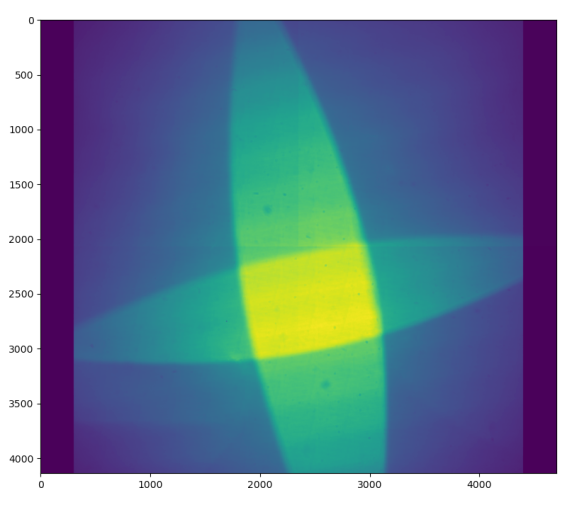
\includegraphics[width=0.3\linewidth]{pics/parent.png}
		\caption{Parent image, prepared by summation of 20 LED images from SUIT.}
		\label{fig:parent}
	\end{figure}
	

	\begin{figure}
		\centering
		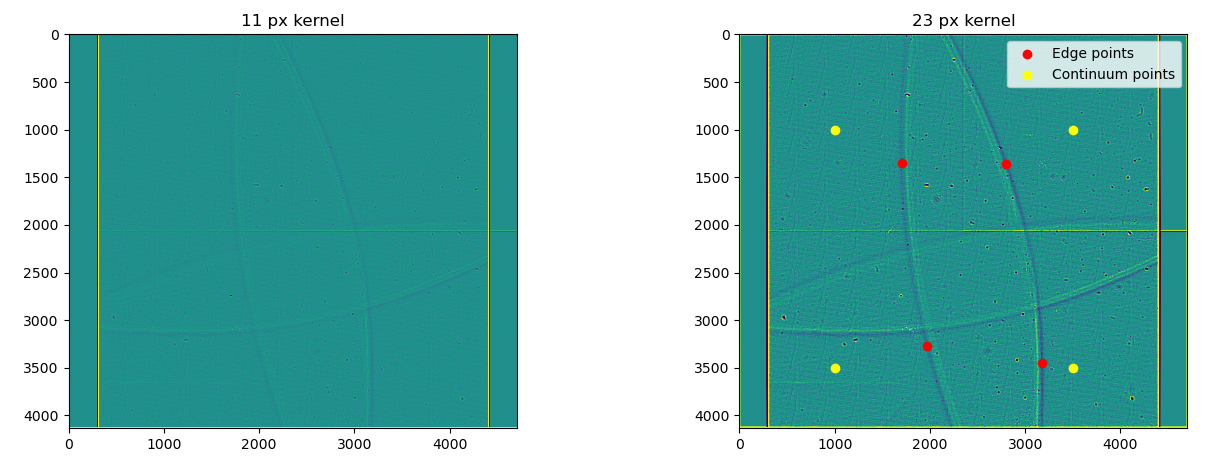
\includegraphics[width=0.8\linewidth]{pics/kernel_compare.png}
		\caption{Comparison of flat field made with kernel size of $11 \times 11$ pixels (Left) and $23 \times 23 $ pixels (Right). Continuum (yellow dots) and Edge (red dots) regions used for mean and standard deviation evaluation are marked in the right panel.}
		\label{fig:kernelcompare}
	\end{figure}

	\begin{figure}
		\centering
		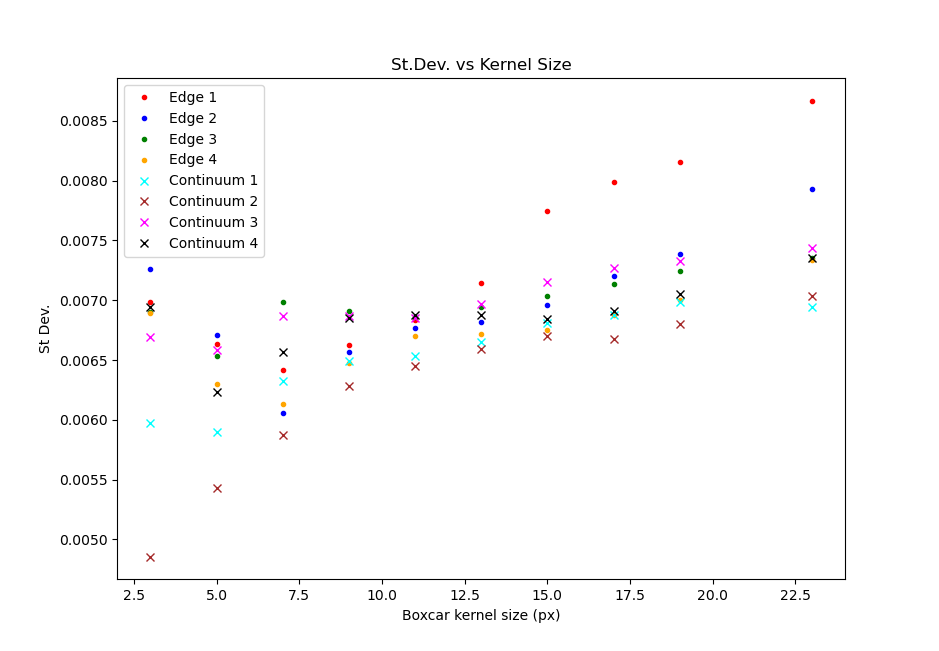
\includegraphics[width=0.9\linewidth]{pics/stdev.png}
		\caption{Standard deviation within kernels of varying sizes at various locations of the flat field image.}
		\label{fig:st}
	\end{figure}

	\begin{figure}
	\centering
	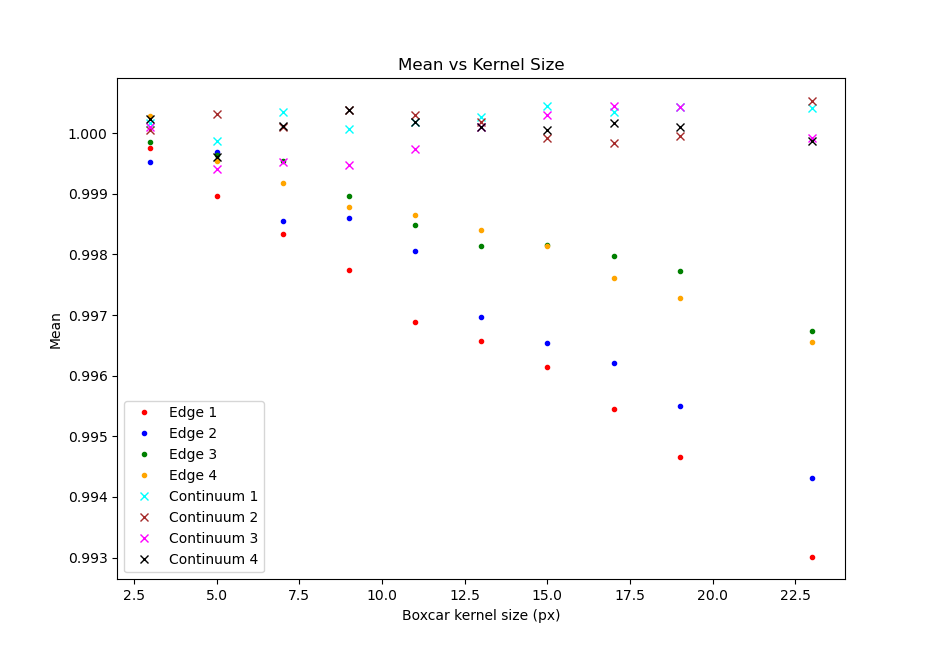
\includegraphics[width=0.9\linewidth]{pics/mean}
	\caption{Mean within kernels of varying sizes at various locations of the flat field image.}
	\label{fig:mean}
	\end{figure}

	\begin{enumerate}
		\item 	20 LED images are recorded using 355 nm on-board LED with SUIT BP3-BB3 science filter combination. These images are summed to get the parent image. 		
		The summation eliminates the contribution of photon noise, read noise etc. to the overall noise. The residual small scale noise is then dominated by pixel to pixel sensitivity variations.  
		
		\item  Flat fields are generated by dividing the parent image by boxcar blurred images with various kernel sizes. For a small kernel, the standard deviation within the kernel is high due greater uncertainty in the measurement of $<k>_{i,j}$ as well as the residual flat field noise. On the other hand, for kernel sizes approaching the edge transition spatial scales, the standard deviations within the Edge regions are high as	the assumption of $S_{i,j} = S$  does not hold well any more. Thus, the residue of the Edge pattern becomes apparent in the flat field image.
		
		\item It is clear from Figure \ref{fig:st} that the standard deviations for both Edge and Continuum regions are tightly clustered at a kernel size of 11x11 pixels. This signifies that the uncertainty in the measurement of $<k>_{i,j}$ is less while ensuring $S_{i,j}=S$ within the kernel. Large scale structures start appearing in the Flat Field upon increasing the kernel size any further.
		
		\item From Figure \ref{fig:mean} we notice that the mean values of the kernels for continuum regions assume a value of 1, as is expected in a flat field image. However, the mean values for Edge regions keep dropping from 1, as the kernel size is increased. This is because the residual of the large scale pattern becomes more prevalent in the flat field image with increasing kernel size.
		
		\item The standard deviation of the mean values at Continuum regions  for 11 pixel kernel is 0.021\% and that for the Edge regions is 0.068\%. These are representative of how much the normalized average flat field estimate deviates from 1 across the image.
	\end{enumerate}
		\section{Evaluation of Flat Field correction process}
			\subsection{Methodology}
					\begin{figure}
				\centering
				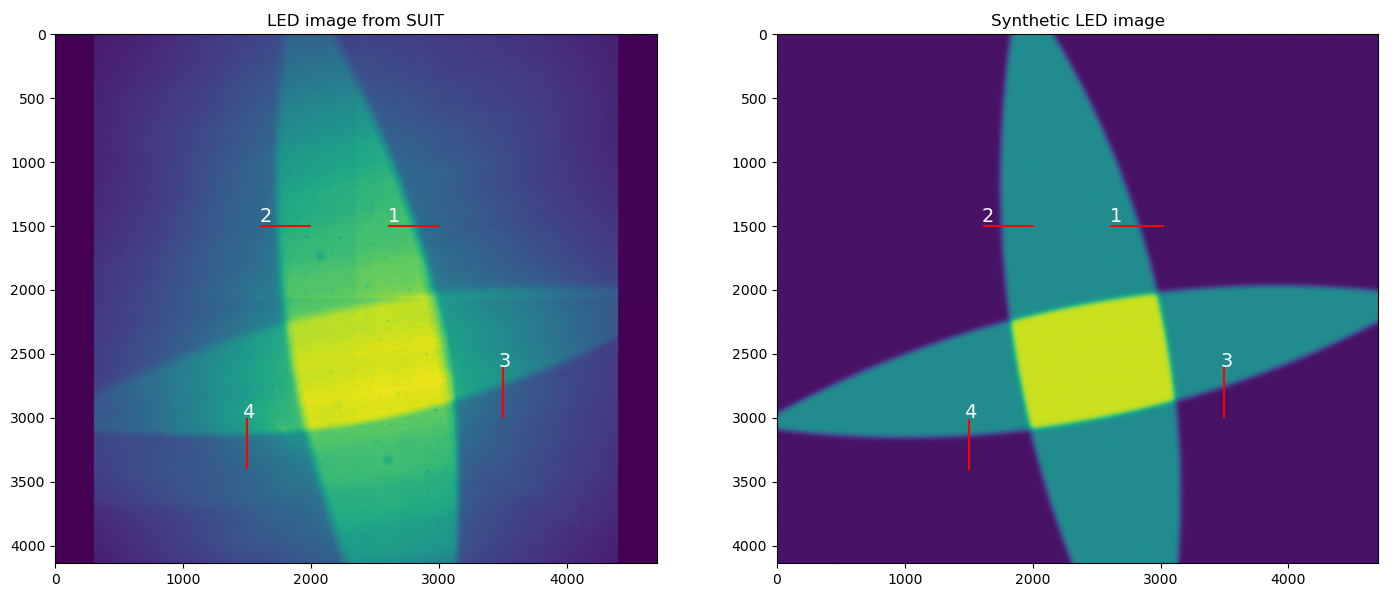
\includegraphics[width=1\linewidth]{pics/image_cuts}
				\caption{Line cut locations on SUIT LED image and synthetic LED image.}
				\label{fig:imagecuts}
				
				\centering
				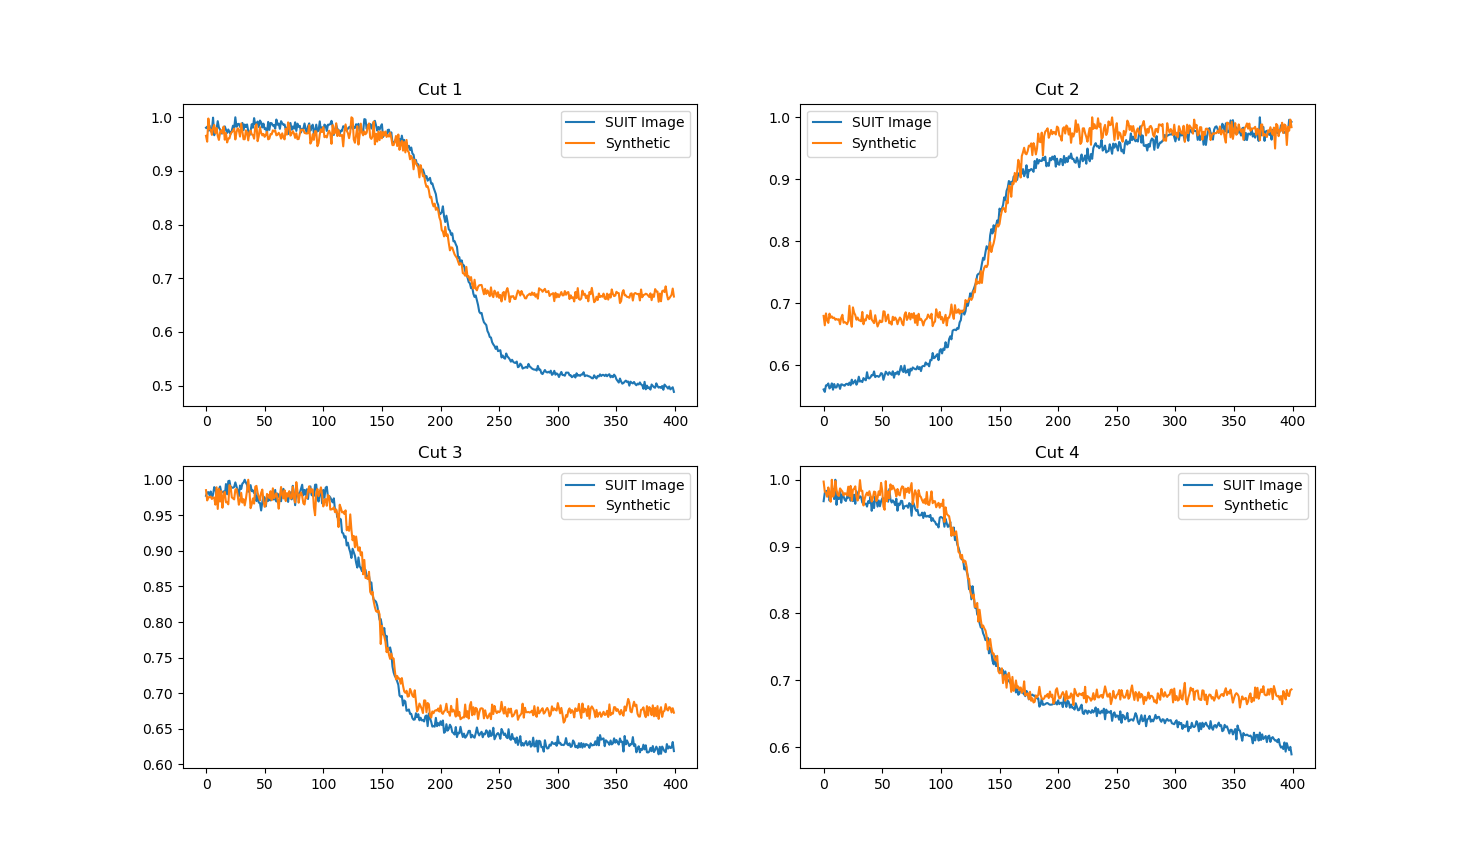
\includegraphics[width=1\linewidth]{pics/cut_plots_synth_p2p_1percent.png}
				\caption{Line cut across a Simulated Image and a Real Image. Performed to compare the extent of blurring applied to smooth the transition at the illumination edges.}
				\label{fig:linecut}
			\end{figure}
			
				\begin{enumerate}
				\item A field with same photoelectron counts is generated for SUIT CCD dimensions of $4704 \times 4136$ px. It is assumed to have $150000 \times 0.9$ photo electrons per pixel, with the factor of 0.9 attributing to 90\% quantum efficiency. This forms the base image.
				
				\item LED illumination pattern, similar to the SUIT LED images is generated. A Gaussian blur with $\sigma=20$ ($\sigma$ controls the extent of blurring) is used to create the blurry effect at the illumination edges. The degree of blurring is compared with line cuts across the simulated image and a real image captured with SUIT as illustrated in  Figures \ref{fig:imagecuts} and \ref{fig:linecut}.
				
				\item \label{p2p} To generate the difference in response from pixel to pixel, a pixel to pixel variation model is generated with a number chosen randomly from a Gaussian distribution of numbers centered at 1, with $\sigma=0.03 (3\%)$. This pixel to pixel variation model is saved for future use. Each pixel of the base image is multiplied with this model to introduce the pixel to pixel variation in the base image. The base image is now subtracted from the modified base image to give the difference introduced in each pixel.
				
				\item \label{shot} To introduce the shot noise, each pixel of the base image is replaced by a randomly chosen number from a Poisson distribution based on the photo electron count of that pixel. The base image is subtracted from the modified image to get the shot noise in each pixel.
				
				\item The differences generated in Points \ref{p2p} and \ref{shot} are added to the base image to implement the pixel to pixel variation and the shot noise. This is repeated for 20 separate images, with the pixel to pixel variation remaining constant, while the shot noise varying in each image. Now we have 20 images with similar illumination, inclusive of pixel to pixel variation and Poisson noise.
				
				\item A field of same dimensions as the image is generated. Each pixel is populated with a randomly drawn number from a Gaussian distribution centered at 7500 with $\sigma= 8$. This corresponds to an offset of 7500 photoelectrons with RMS read noise of 8 photo electrons. This field is generated uniquely and each unique image is added to each of the 20 generated LED images.
				
				\item The images are divided by a gain factor of 3 to get the equivalent ADC counts and bias value of 2500 (7500 photo electrons / 3) is subtracted to get the final images.
				
				\item The generated images are run through the developed flat field correction mechanism and the results are compared with a synthetic image inclusive of all noises, but devoid of any pixel-to-pixel variation.
				
				\item A synthetic Sun-like image is also generated with Poisson noise and Read noise. One version of the image is inclusive of the pixel-to-pixel variation as in Figure \ref{fig:syntheticsun}. This image is run through the flat field correction mechanism and the results are compared with a version of the image devoid of any pixel-to-pixel variation.
				
				\item Here, the evaluations have been performed in a pixel-wise fashion. However, in practice, the photometry of the Sun would be limited by the size of the PSF. Therefore, a realistic case is developed where standard deviations of the mean values of $4\times4 px$, similar to SUIT PSF, are used for the evaluation of residual flat field error. 
			\end{enumerate}
		
		
%%	\begin{figure}
	%	\centering
	%	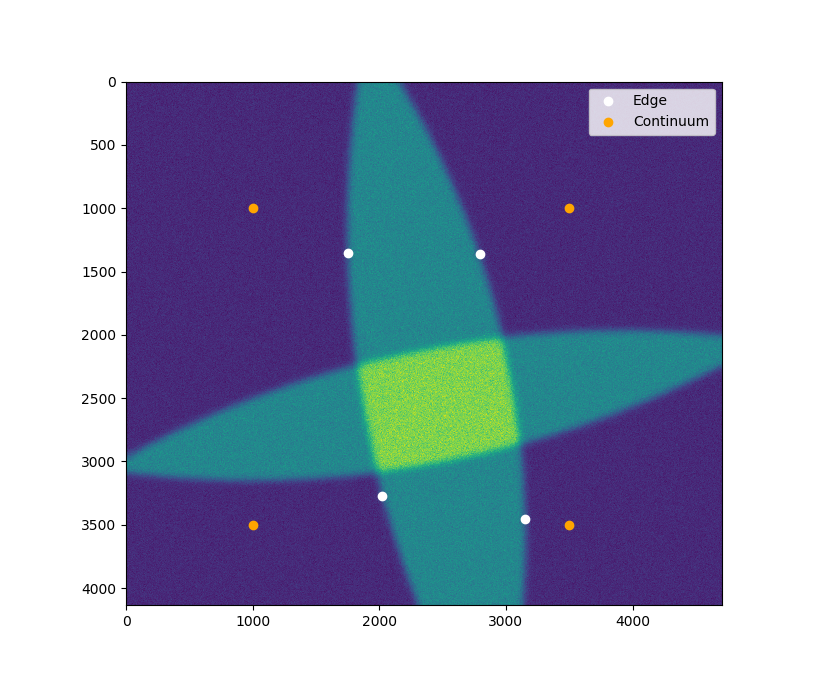
\includegraphics[width=0.6\linewidth]{pics/locations.png}
	%	\caption{Locations of Edge and Continuum regions chosen for evaluation of Mean and Standard Deviations within kernels of various sizes.}
%		\label{fig:locations}
%	\end{figure}
	
	\subsection{Results}
	\begin{figure}
		\centering
		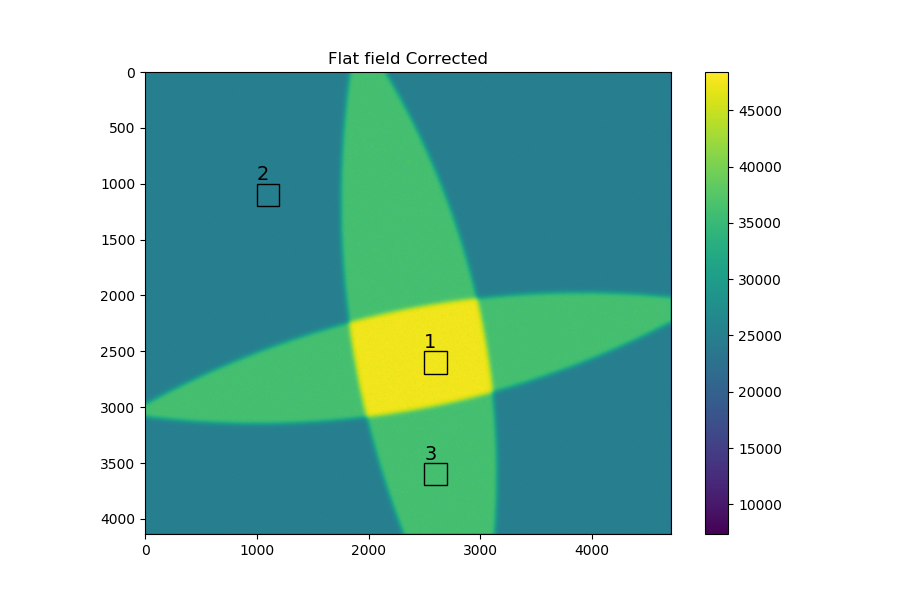
\includegraphics[width=0.6\linewidth]{pics/analysis_locations.png}
		\caption{Box locations chosen for analysis on Flat Field Corrected synthetic image.}
		\label{fig:analysislocations}
	\end{figure}
	
	\begin{table}
		\centering
		\begin{tabular}{|c|c|c|c|}
			\hline
			\textbf{Parameter} &\textbf{ Location 1 }&\textbf{ Location 2} & \textbf{Location 3} \\ 
			\hline
			\hline 
			\multicolumn{4}{|c|}{\textit{Synthetic LED Image}} \\ 
			\hline
			\hline 
			\textit{St. Dev.} $(\sigma_1)$ &1363  & 684 & 1013 \\ 
			\hline 
			\textit{Mean }$(\mu_1)$& 44999 & 22505 & 33746 \\ 
			\hline 
			\textit{\% St. Dev.} &3.03  & 3.04 & 3.00 \\ 
			\hline 
			\hline
			\multicolumn{4}{|c|}{\textit{Synthetic LED Image without px to px variation}} \\ 
			\hline
			\hline 
			\textit{St. Dev.} $(\sigma_2)$&122  & 87 & 105 \\ 
			\hline 
			\textit{Mean} $(\mu_2)$& 45000 & 22500 & 33750 \\ 
			\hline 
			\textit{\% St. Dev.}& 0.27 & 0.38 & 0.31 \\ 
			\hline 
			\hline
			\multicolumn{4}{|c|}{\textit{Flat Corrected Synthetic LED Image}} \\ 
			\hline
			\hline 
			\textit{St. Dev. }$(\sigma_3)$& 171 & 104 & 138 \\ 
			\hline 
			\textit{Mean} $(\mu_3)$& 44999 & 22506 & 33745 \\ 
			\hline 
			\textit{\% St. Dev.}& 0.39 & 0.46 & 0.41 \\ 
			\hline 
			\hline
			\multicolumn{4}{|c|}{\textit{Residual \% Error in Flat Field} $\left(\dfrac{\sqrt{\sigma_3^2-\sigma_2^2}}{\mu_2}\right)$} \\
			\hline
			\hline
			& 0.27 & 0.25 & 0.26 \\ 
			\hline
		\end{tabular} 
		\caption{Noise levels in synthetic LED images and residual error in flat field estimation. Locations marked in Figure \ref{fig:analysislocations}. }
		\label{table:compare}
	\end{table}


	\begin{figure}
		\begin{subfigure}[b]{0.49\textwidth}
			\centering
			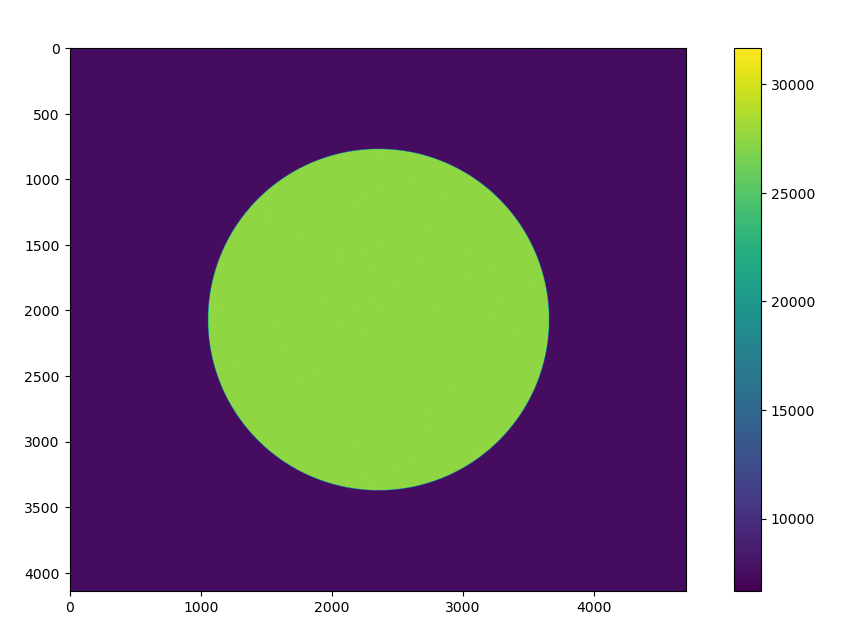
\includegraphics[width=\textwidth]{pics/synthetic_sun}
			\caption{Expected image of Sun through SUIT.}
			\label{fig:syntheticsun}
		\end{subfigure}
	\hfill
		\begin{subfigure}[b]{0.48\textwidth}
	\centering
	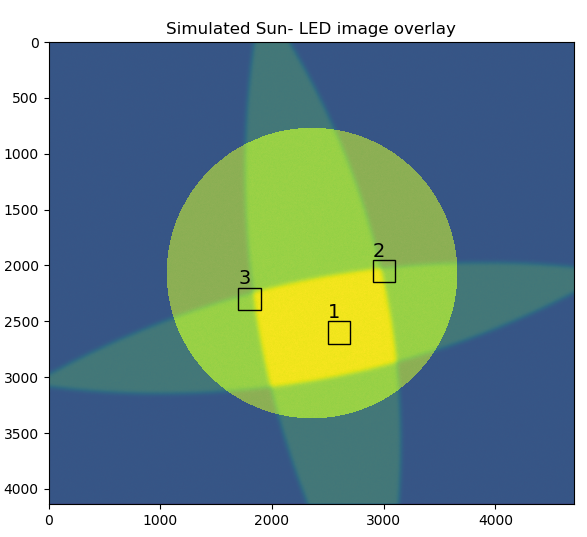
\includegraphics[width=0.8\textwidth]{pics/sun_Locations.png}
	\caption{LED pattern overlaid to illustrate the chosen analysis regions.}
	\label{fig:sunlocations}
	\end{subfigure}
	\caption{Synthetic image of the Sun comprising of pixel-to-pixel variation with poission and read noises.}
	\end{figure}
	

	\begin{enumerate}
		\item To test the validity of our flat field correction methodology, the generated images are run through the flat field correction pipeline. The standard deviation over $200 \times 200$ pixel regions are compared between a Synthetic LED image, a flat field corrected image and an image devoid of pixel to pixel variation but having Poission and Read noises. The evaluation is done at 3 locations across the image which are illustrated in Figure \ref{fig:analysislocations} and tabulated in Table \ref{table:compare}.

		\item The \% standard deviation of the Synthetic LED Image within the analysis boxes are $\approx 3\%$ of their means. This shows that the noise due to pixel to pixel variation, along with Poisson and read noises is $\approx 3\%$.
		
		\item The \% standard deviation of the Synthetic LED Image without Pixel to Pixel variation within the analysis boxes are $\approx 0.3\%$ with respect to their mean values due to Poisson and Read noises.
		
		\item The \% standard deviation of the Flat field corrected Synthetic LED Image within the analysis boxes are $\approx 0.4\%$ of their mean values. Thus the contribution of all noises, after correction of pixel to pixel variation is $\approx 0.4\%$.
		
		\item The residual flat field error calculated as per Table \ref{table:compare} is $\approx 0.26\%$ which is much lesser than the required $1\%$. This signifies that the flat field correction mechanism is effectively correcting for pixel to pixel response variations in the image.
		
		\item The same methodology is followed for flat field correction of a synthetic sun like image. The $200\times200 px$ boxes chosen for analysis are illustrated in Figure \ref{fig:sunlocations}. The results of the analysis are tabulated in Table \ref{table:suncompare}. The LED illumination pattern is overlaid on Figure \ref{fig:sunlocations} for ease of understanding.
		
		\item The residual \% error in flat field estimation is $\approx 0.3\%$, which is much lesser than the 1\% limit in both the Edge region as well as a continuum region of the large scale LED pattern within the solar disk. Thus, we can conclude that the flat field correction mechanism effectively rectifies the pixel to pixel variation.
		
		\item The standard deviation and mean within kernels of varying sizes are computed at four Edge and four Continuum regions in the generated flat field image at the same locations as illustrated in Figure \ref{fig:kernelcompare}.
		
		\item \label{point:stdev} From Figure \ref{fig:synth_st} we notice that the standard deviations for continuum and edge regions get clustered for kernel size of $\approx 14\times 14 px$ before diverging. 
		\begin{enumerate}
		\item With small kernel sizes, the standard deviation of the continuum and edge regions are high. So all the points in the plot appear scattered.
		
		\item As kernel size increases, the points due to the Edge and the points due to the Continuum regions get clustered among themselves.
		
		\item It is noticed that the continuum region clusters assume a value of $\approx 0.03$, as expected due to the 3\% pixel to pixel variation. However, the clusters for the Edge regions appear to diverge as residues of the large scale patterns start appearing in the generated flat field images for higher kernel sizes.
		
		\item The point where all the continuum and edge points appear to closely cluster is therefore the sweet spot where the kernel is large enough to gather sufficient number of pixels to generate a reliable flat field, while not so large as to pick up the large scale pattern.
		\end{enumerate}
		
		\item \label{point:Mean}It is noticed from Figure \ref{fig:synth_mean} that the mean value within the kernels drop rapidly beyond $\approx 14 px$ for Edge regions, while they cluster around 1 for continuum regions.
		\begin{enumerate}
			\item At small kernel sizes, the mean values within the kernels are equally scattered due to greater uncertainty in the determination of the mean.
			\item At larger kernel sizes, the mean values for edge regions and the mean values for Continuum regions appear to cluster among themselves. This happens as the certainty in the mean determination increases.
			\item At large kernel sizes, the mean values at the continuum regions appear to assume a value of 1. This also signifies that the variation of counts among the pixels in these regions are centered at 1, as expected from a flat field with pixel-to-pixel variations only.
			\item At large kernel sizes, the mean values of the Edge regions drop systematically as the large scale pattern starts showing up in the flat field as a residue.
			\item The mean values of the Edge regions tend to separate themselves from the Continuum region mean values at a kernel size of $\approx 14\times14 px$.
		\end{enumerate}
	
	\item Here, the evaluations have been performed in a pixel-wise fashion. However, in practice, the photometry of the Sun would be limited by the size of the PSF. This is simulated by taking average of $4 \times 4$ pixels as one photometric unit.
	\begin{enumerate}
		\item 50 such $4\times4$ boxes are chosen randomly from the flat field corrected solar disc image. The points are marked in Figure \ref{fig:sunphotometry}.
		\item The mean of each point is evaluated to get the photometric intensity within the PSF.
		\item The ratio of the standard deviation ($\sigma= 62.7$ ) and mean ($\mu= 25010.6$) of these points signify the extent of residual error present in the corrected image.
		\item The \% residual error is $\dfrac{\sigma}{\mu}*100\%= 0.25\%$. This is much lesser than the upper limit of 1\%.
	\end{enumerate}
	\end{enumerate}
	
	\begin{table}
		\centering
		\begin{tabular}{|c|c|c|c|}
			\hline
			\textbf{Parameter} &\textbf{ Location 1 }&\textbf{ Location 2} & \textbf{Location 3} \\ 
			\hline
			\hline 
			\multicolumn{4}{|c|}{\textit{Synthetic Sun Image }} \\ 
			\hline
			\hline 
			\textit{St. Dev.} $(\sigma_1)$ &760.4  & 756.0 & 755.5 \\ 
			\hline 
			\textit{Mean }$(\mu_1)$& 25000.5 & 24997.9 & 25000.1 \\ 
			\hline 
			\textit{\% St. Dev.} &3.04  & 3.03 & 3.02 \\ 
			\hline 
			\hline
			\multicolumn{4}{|c|}{\textit{Synthetic Sun Image without px to px variation}} \\ 
			\hline
			\hline 
			\textit{St. Dev.} $(\sigma_2)$& 90.7  & 91 & 91.5 \\ 
			\hline 
			\textit{Mean} $(\mu_2)$& 24999.6 & 25000.1 & 25000.3 \\ 
			\hline 
			\textit{\% St. Dev.}& 0.36 & 0.37 & 0.36 \\ 
			\hline 
			\hline
			\multicolumn{4}{|c|}{\textit{Flat Corrected Synthetic Sun Image}} \\ 
			\hline
			\hline 
			\textit{St. Dev. }$(\sigma_3)$& 115.5 & 116.0 & 117.1 \\ 
			\hline 
			\textit{Mean} $(\mu_3)$& 25000.5 & 25000.7 & 25001.5 \\ 
			\hline 
			\textit{\% St. Dev.}& 0.46 & 0.46 & 0.47 \\ 
			\hline 
			\hline
			\multicolumn{4}{|c|}{\textit{Residual \% Error in flat field} $\left(\dfrac{\sqrt{\sigma_3^2-\sigma_2^2}}{\mu_2}\right)$} \\
			\hline
			\hline
			& 0.28 & 0.29 & 0.30 \\ 
			\hline
		\end{tabular}
		\caption{Noise levels in synthetic Sun images and residual error in flat field estimation. Locations marked in Figure \ref{fig:sunlocations}. }
		\label{table:suncompare}
	\end{table}
	
	
	\begin{figure}
		\centering
		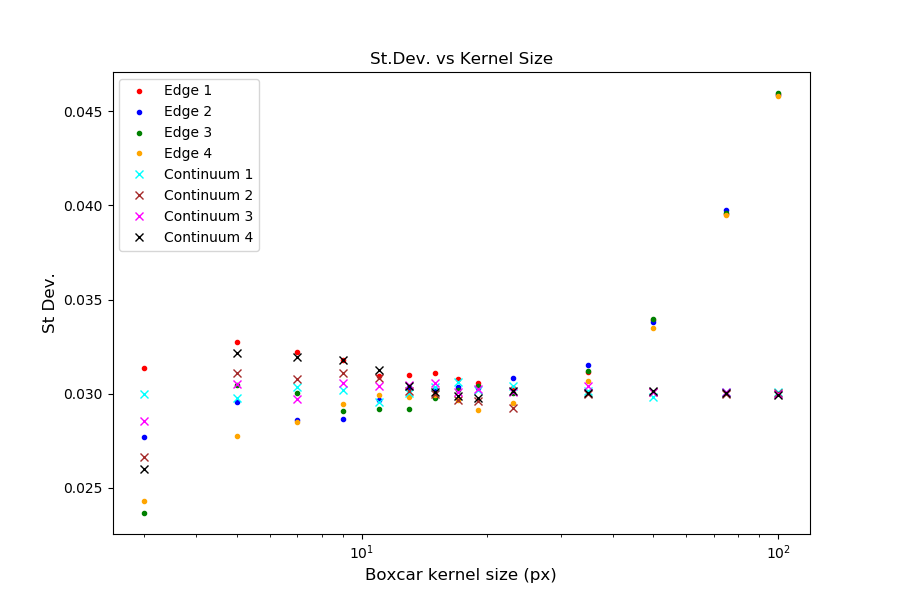
\includegraphics[width=0.8\linewidth]{pics/synth_Stdev.png}
		\caption{Standard deviation within kernels of varying sizes at various locations of the flat field image.}
		\label{fig:synth_st}
	\end{figure}
	
	
	\begin{figure}
		\centering
		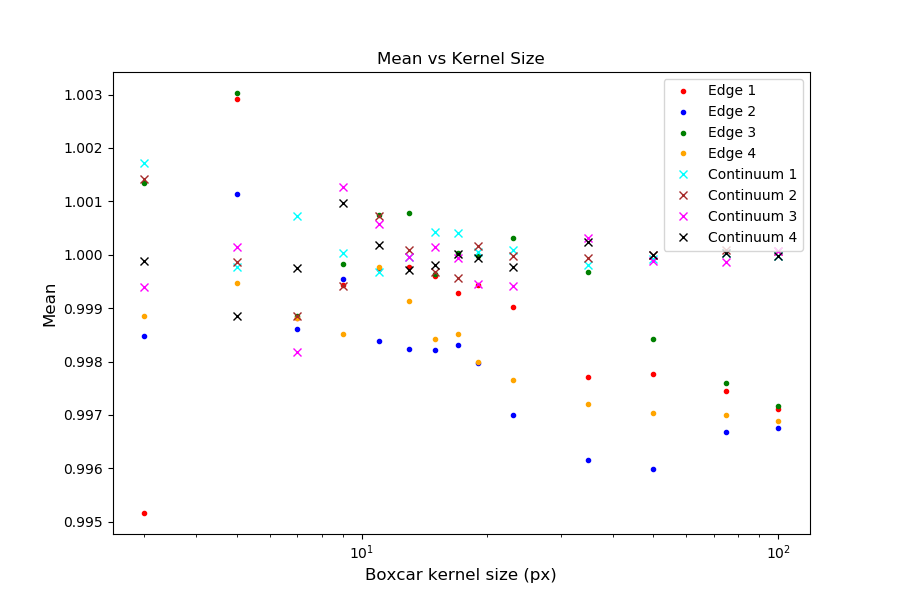
\includegraphics[width=0.8\linewidth]{pics/synth_Mean.png}
		\caption{Mean within kernels of varying sizes at various locations of the flat field image.}
		\label{fig:synth_mean}
	\end{figure}

	\begin{figure}
		\centering
		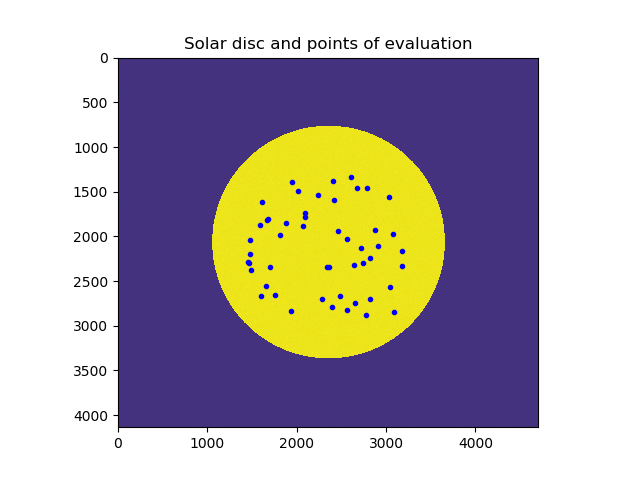
\includegraphics[width=0.7\linewidth]{pics/sun_photometry}
		\caption{Randomly chosen points marked on flat corrected synthetic Sun image.}
		\label{fig:sunphotometry}
	\end{figure}
	

	\section{Conclusion}
		In this document we established the methodology for correction of pixel to pixel variation in SUIT images with the aid of on board LEDs. This is achieved by removing large scale illumination pattern from the images while preserving the pixel to pixel variation in response. 
		
		The developed methodology is tested on synthetically generated LED images with known levels of Poisson noise, read noise and pixel-to-pixel response variation. This is also tested with a Sun-like image comprising of all the above noises. It is noticed that the residual flat field error is $\approx 0.26\%$ for the former and $\approx 0.29 \%$ for the latter. The residual errors are well within our requirement of 1\% photometric accuracy.
		
		Finally, a realistic scenario is developed with the knowledge of SUIT PSF occupying an area of $4\times4$ pixels. The residual error seen in this test is $0.25\%$, much lesser than our upper limit of 1\%.
		
		Therefore, we can conclude that the SUIT flat field generation mechanism for correction of pixel-to-pixel response variation is robust and can be implemented on solar data produced by SUIT.


\begin{center}
	-x-
\end{center}

\end{document}